% REFERENCIAL TEORICO---------------------------------------------------

\chapter{RESULTADO}
\label{chap:introducao}

Neste capitulo, serão detalhados os resultados obtidos nas telas da aplicação móvel, e também o resultado obtido no desenvolvimento da API. Na aplicação móvel, vão ser abordados assuntos como acessibilidade, usabilidade e a experiência do usuario. já na API, seram detalhadas as rotas criadas, bem como a documentação preparada.

\section{INTERFACE DE PROGRAMAÇÃO DE APLICAÇÕES}
\label{sec:resultadoApi}

Para documentar e descrever com clareza as rotas, a documentação Swagger foi utilizada. Segundo a documentação do \citeonline{SwaggerDoc2025}, tal produto visa criar uma documentação automática utilizando definições diretas da API, mantendo consistência e confiabilidade.. A \autoref{fig:docSwaggerAPI} exibe parte da documentação WEB gerada pela biblioteca Swagger istalada e configurada no projeto FishSpotAPI, nela é possivel realizar requisições HTTP, utilizar recursos de autenticação, e visualizar quais esquemas são usados nas requisições.

\begin{figure}[H]
    \centering
    \caption{Documentação Swagger - Rota de Autenticação}
    \label{fig:docSwaggerAPI}
    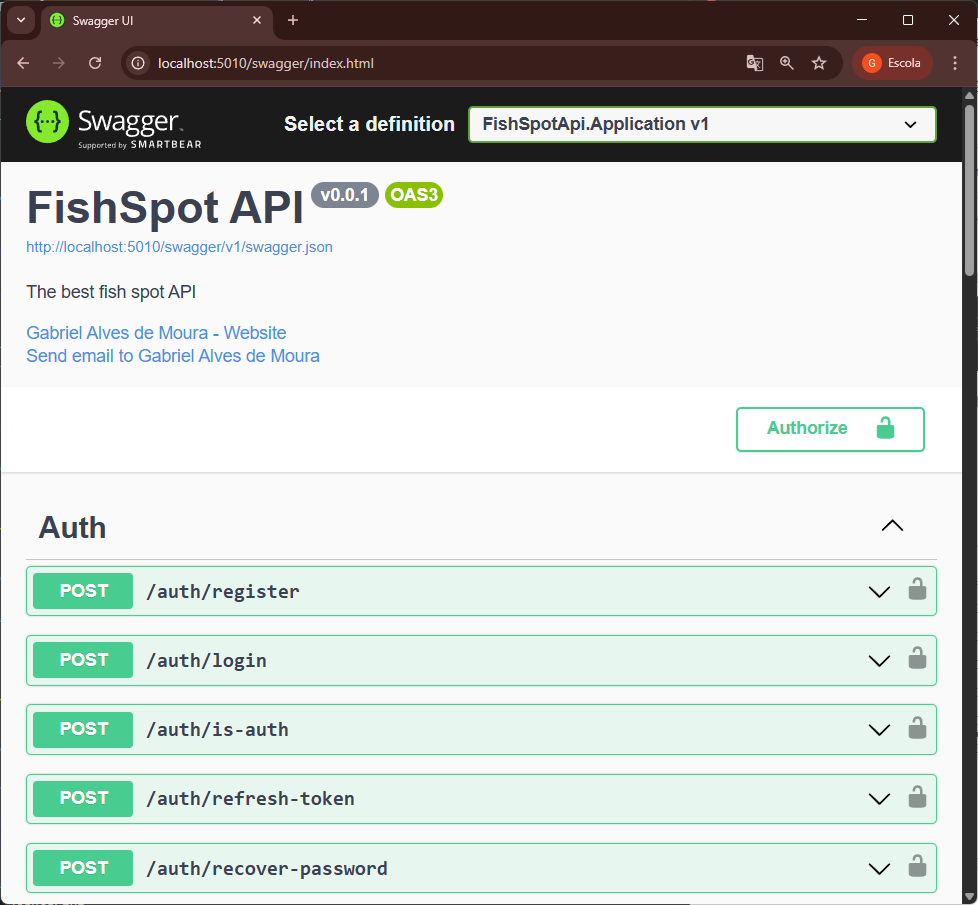
\includegraphics[scale=0.53]{./dados/figuras/api-swagger.png}
    \fonte{Produzido pelo Autor}
\end{figure}

A \autoref{fig:docSwaggerOthersAPI} exibe outra parte da documentação WEB gerada pela biblioteca Swagger istalada e configurada no projeto. Nesta parte exibida, podemos observar as rotas de recursos, de ponto de pesca e tambem de usuário.

\begin{figure}[H]
    \centering
    \caption{Documentação Swagger - Rota de Recursos, Ponto de Pesca e Usuário}
    \label{fig:docSwaggerOthersAPI}
    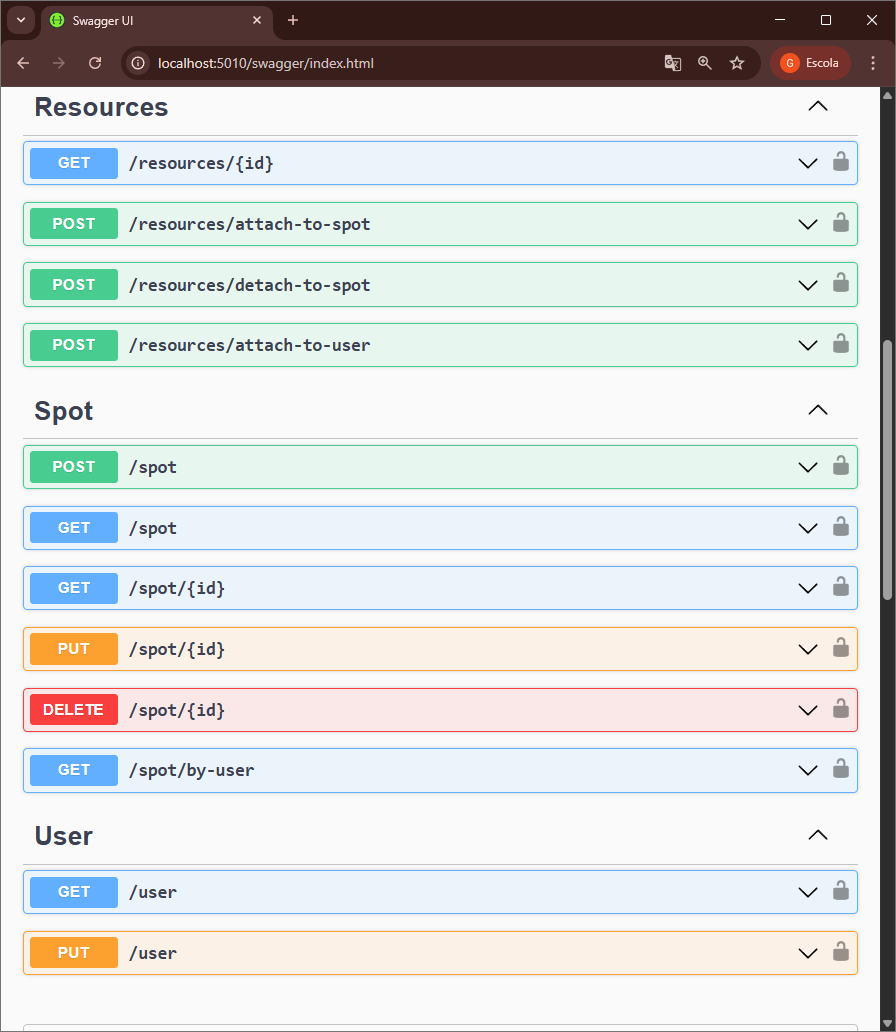
\includegraphics[scale=0.60]{./dados/figuras/swagger-api-others.png}
    \fonte{Produzido pelo Autor}
\end{figure}

\newpage

Pode-se observar na \autoref{fig:docSwaggerLoginAPI} o componente que pode ser usado para fazer uma requisição HTTP para a rota de Login. É possivel visualizar que é possivel incluir um corpo, parametros e visualizar qual o resultado obtido no final.

\begin{figure}[H]
    \centering
    \caption{Documentação Swagger - Documentação da Rota de Login}
    \label{fig:docSwaggerLoginAPI}
    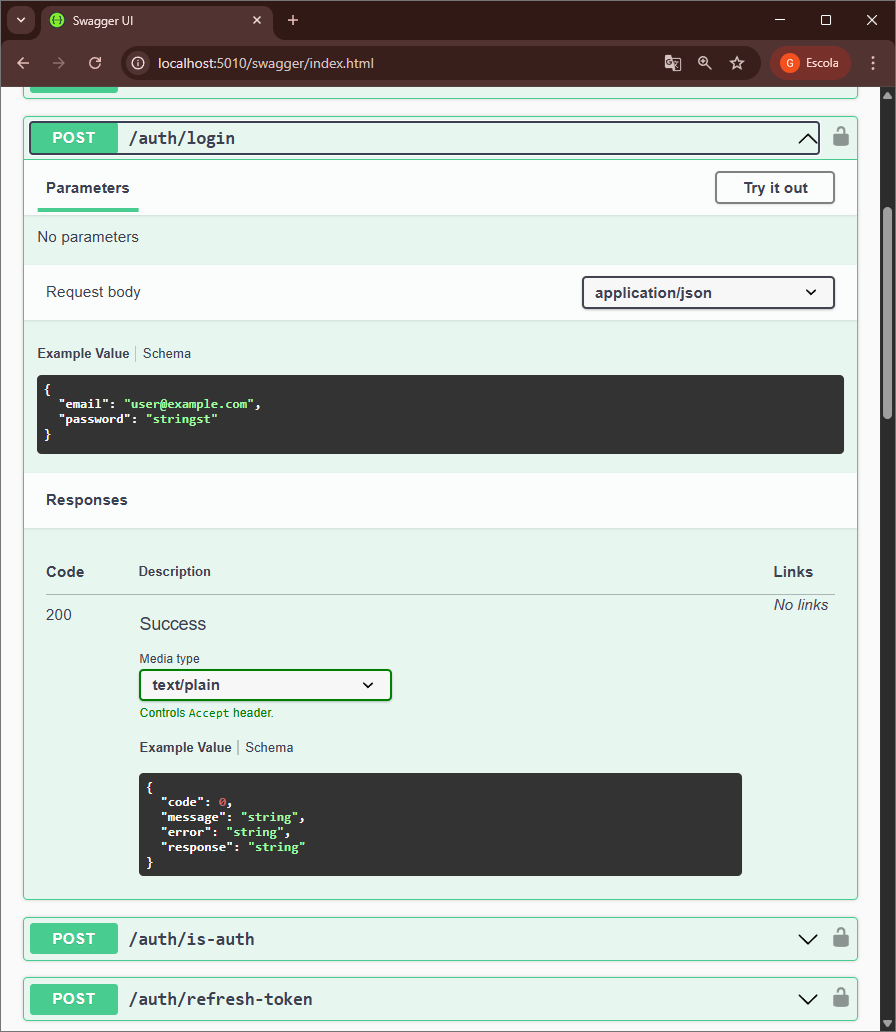
\includegraphics[scale=0.60]{./dados/figuras/swagger-api-login-doc.png}
    \fonte{Produzido pelo Autor}
\end{figure}


\newpage

A \autoref{tab:tb-api-fishspot} e a \autoref{tab:tb-api-fishspot-others},  apresentam de forma simples todos os endereços disponiveis na interface de programação de aplicações do ambiente FishSpot. Ela contem o método HTTP que deve ser utilizado na requisição, qual o endereço que deve ser utilizado e uma breve descrição de qual a funcionalidade da rota.

\begin{table}[h!]
    \centering
    \caption[Rotas Disponiveis]{Rotas Disponiveis
    \label{tab:tb-api-fishspot}}
    \setlength{\extrarowheight}{4pt}
    \begin{tabular}{|c|l|p{0.35\textwidth}|} 
        \hline
        \multicolumn{3}{|c|}{\textbf{Autenticação}} \\
        \hline
        \textbf{Método HTTP} & \textbf{Endereço da Rota} & \textbf{Detalhes} \\
        \hline
        POST & /auth/register & Registrar usuário no sistema \\
        \hline
        POST & /auth/login & Autenticar usuário no sistema \\
        \hline
        POST & /auth/is-auth & Valida se o usuário esta autenticado, e consegue usar todos os recursos disponiveis \\
        \hline
        POST & /auth/recover-password & Notifica o sistema que o usuário quer alterar a senha \\
        \hline
        POST & /auth/validate-recover-token & Valida o token recebido por outros meios pelo usuário \\
        \hline
        POST & /auth/change-password & Altera a senha do usuário \\
        \hline

        % Recursos ---------------

        \multicolumn{3}{|c|}{\textbf{Recursos (Fotos, Imagem e etc)}} \\
        \hline
        \textbf{Método HTTP} & \textbf{Endereço da Rota} & \textbf{Detalhes} \\
        \hline
        GET & /resources/\{id\} & Consultar na aplicação o recurso relacionado ao identificador informado \\
        \hline
        POST & /resources/attach-to-spot & Anexar fotos ou imagens ao ponto de pesca \\
        \hline
        POST & /resources/detach-to-spot & Desanexar fotos ou imagens do ponto de pesca \\
        \hline
        POST & /resources/attach-to-user & Anexar foto ao perfil do usuário \\
        \hline

        % Gerenciar Usuario ------------ 

        \multicolumn{3}{|c|}{\textbf{Usuário (Gerenciar Dados)}} \\
        \hline
        \textbf{Método HTTP} & \textbf{Endereço da Rota} & \textbf{Detalhes} \\
        \hline
        GET & /user & Consultar os dados não sensiveis do usuario \\
        \hline
        PUT & /user & Alterar os dados do usuário \\
        \hline

    \end{tabular}
    \fonte{Fonte: Produzido pelo Autor}
\end{table}



\begin{table}[h!]
    \centering
    \caption[Rotas Disponiveis Continuação]{Rotas Disponiveis Continuação
    \label{tab:tb-api-fishspot-others}}
    \setlength{\extrarowheight}{4pt}
    \begin{tabular}{|c|l|p{0.35\textwidth}|} 

        % Ponto de Pesca ---------------
        \hline
        \multicolumn{3}{|c|}{\textbf{Ponto de Pesca}} \\
        \hline
        \textbf{Método HTTP} & \textbf{Endereço da Rota} & \textbf{Detalhes} \\
        \hline
        POST & /spot & Criar um ponto de pesca com base nos dados recebidos \\
        \hline
        GET & /spot & Consultar pontos de pesca cadastrados no sistema \\
        \hline
        GET & /spot/\{id\} & Consultar um ponto de pesca específico com base no identificador recebido \\
        \hline
        PUT & /spot/\{id\} & Alterar os dados de um ponto de pesca específico com base no identificador recebido \\
        \hline
        DELETE & /spot/\{id\} & Remover um ponto de pesca específico com base no identificador recebido \\
        \hline
        GET & /spot/by-user & Consultar os pontos de pesca com base no usuário autenticado \\
        \hline
        
    \end{tabular}
    \fonte{Fonte: Produzido pelo Autor}
\end{table}

\newpage

\section{APLICATIVO MÓVEL}
\label{sec:desenvolvimentodoapp}

Os resultados obtidos do desenvolvimento da aplicação desenvolvida utilizando o framework Flutter, serão detalhados neste capitulo. O resultado obtido segue o protótipo proposto e já descrito neste documento; entretanto, algumas alterações foram necessárias devido à falta de conhecimento em aplicações móveis no quesito responsividade.

Uma das partes que precisou de ajustes para se adaptar à responsividade foi o componente de detalhes do ponto de pesca. Originalmente prototipado com abas (ou guias) laterais, ele foi redesenhado e implementado como uma lista. Outra parte que exigiu ajustes foi o componente de entrada de texto, que demandava maior proficiência no desenvolvimento com o framework Flutter.

Nas figuras é possivel observar utilização de um mapa com visual diferente dos conhecidos (Google Maps, Waze, Uber e etc), essa diferença é devido ao uso do OpenStreetMap uma plataforma de mapas aberta a comunidade, onde os membros são responsáveis por editar as ruas, avenidas, estradas e etc. Tal plataforma é matida pelo grupo \citeonline{OpenStreetMap}, e por efeito do uso do OSM, é necessário que os direitos autorais sejam atribuídos, como documentado pela página oficial.

% ---- Modo Escuro

A \autoref{fig:emultatorAuthPages} mostra o resultado obtido do desenvolvimento das telas relacionadas a autenticação do pescador no modo escuro. Dentre as páginas desenvolvidas, estão as páginas de autenticação, registro e recuperação de senha.

\begin{figure}[H]
    \centering
    \caption{Resultado Obtido - Telas de Autenticação}
    \label{fig:emultatorAuthPages}
    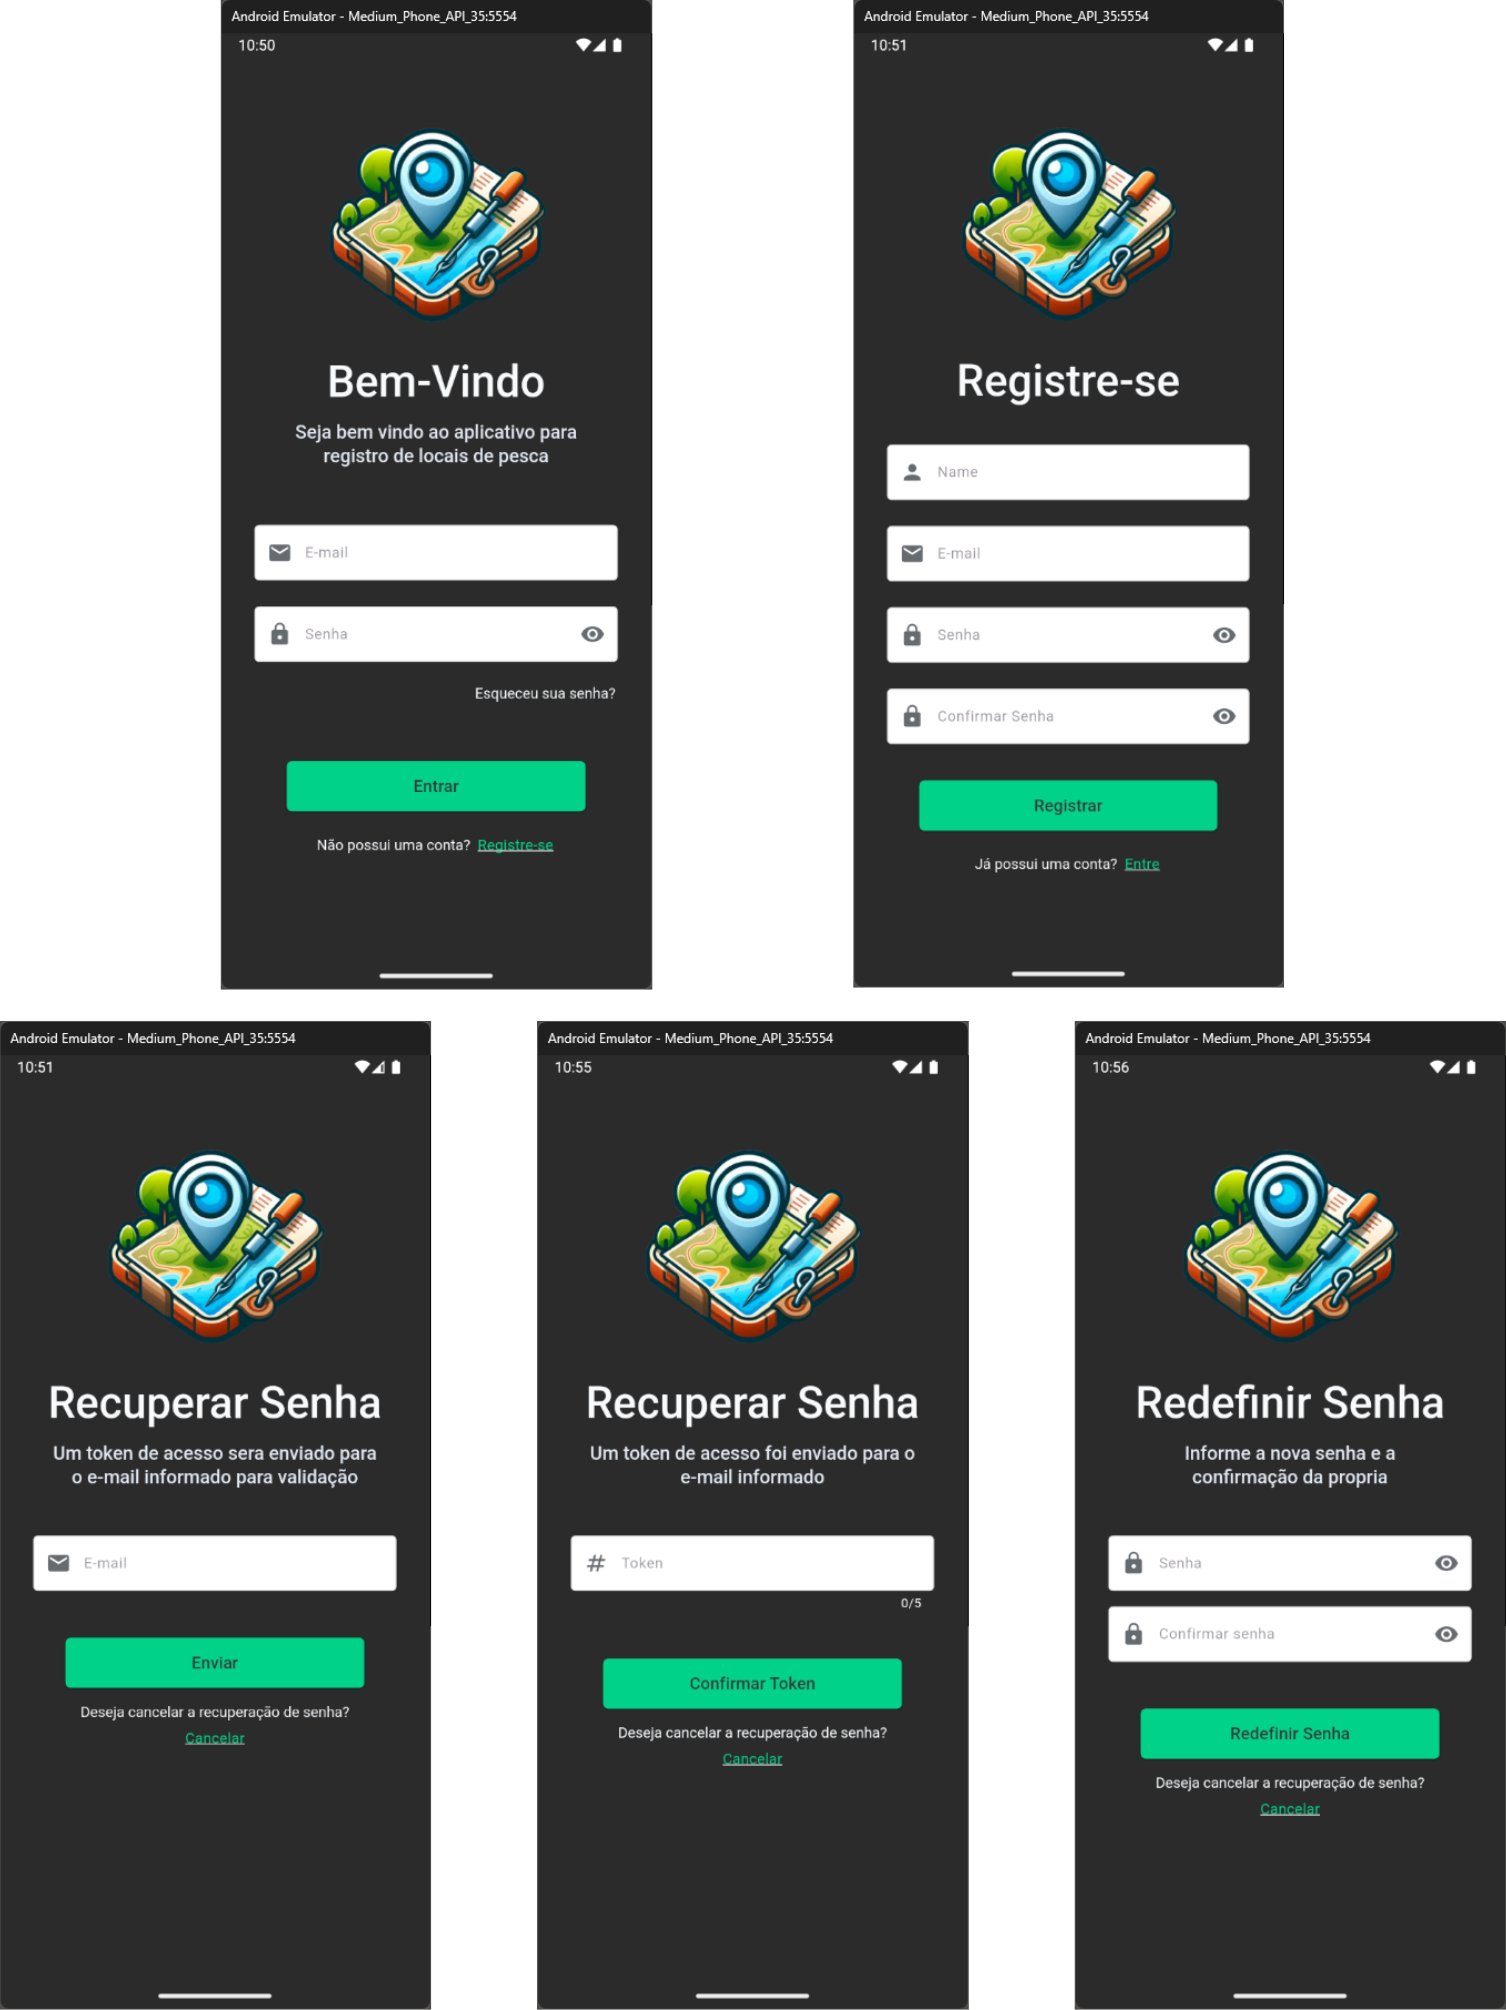
\includegraphics[scale=0.35]{./dados/figuras/emulator-auth-pages.png}
    \fonte{Produzido pelo Autor}
\end{figure}


As telas relacionadas ao mapa principal e aos detalhes dos usuário, tal qual um perfil de usuário, estão sendo representadas pela \autoref{fig:emultatorMapAndPerfilPages}. A figura mostra as páginas desenvolvidas no modo escuro, as quais proporcionam qualidade de observação duranto o uso do aplicativo para os usuários.

\begin{figure}[H]
    \centering
    \caption{Resultado Obtido - Telas de Mapa e Perfil}
    \label{fig:emultatorMapAndPerfilPages}
    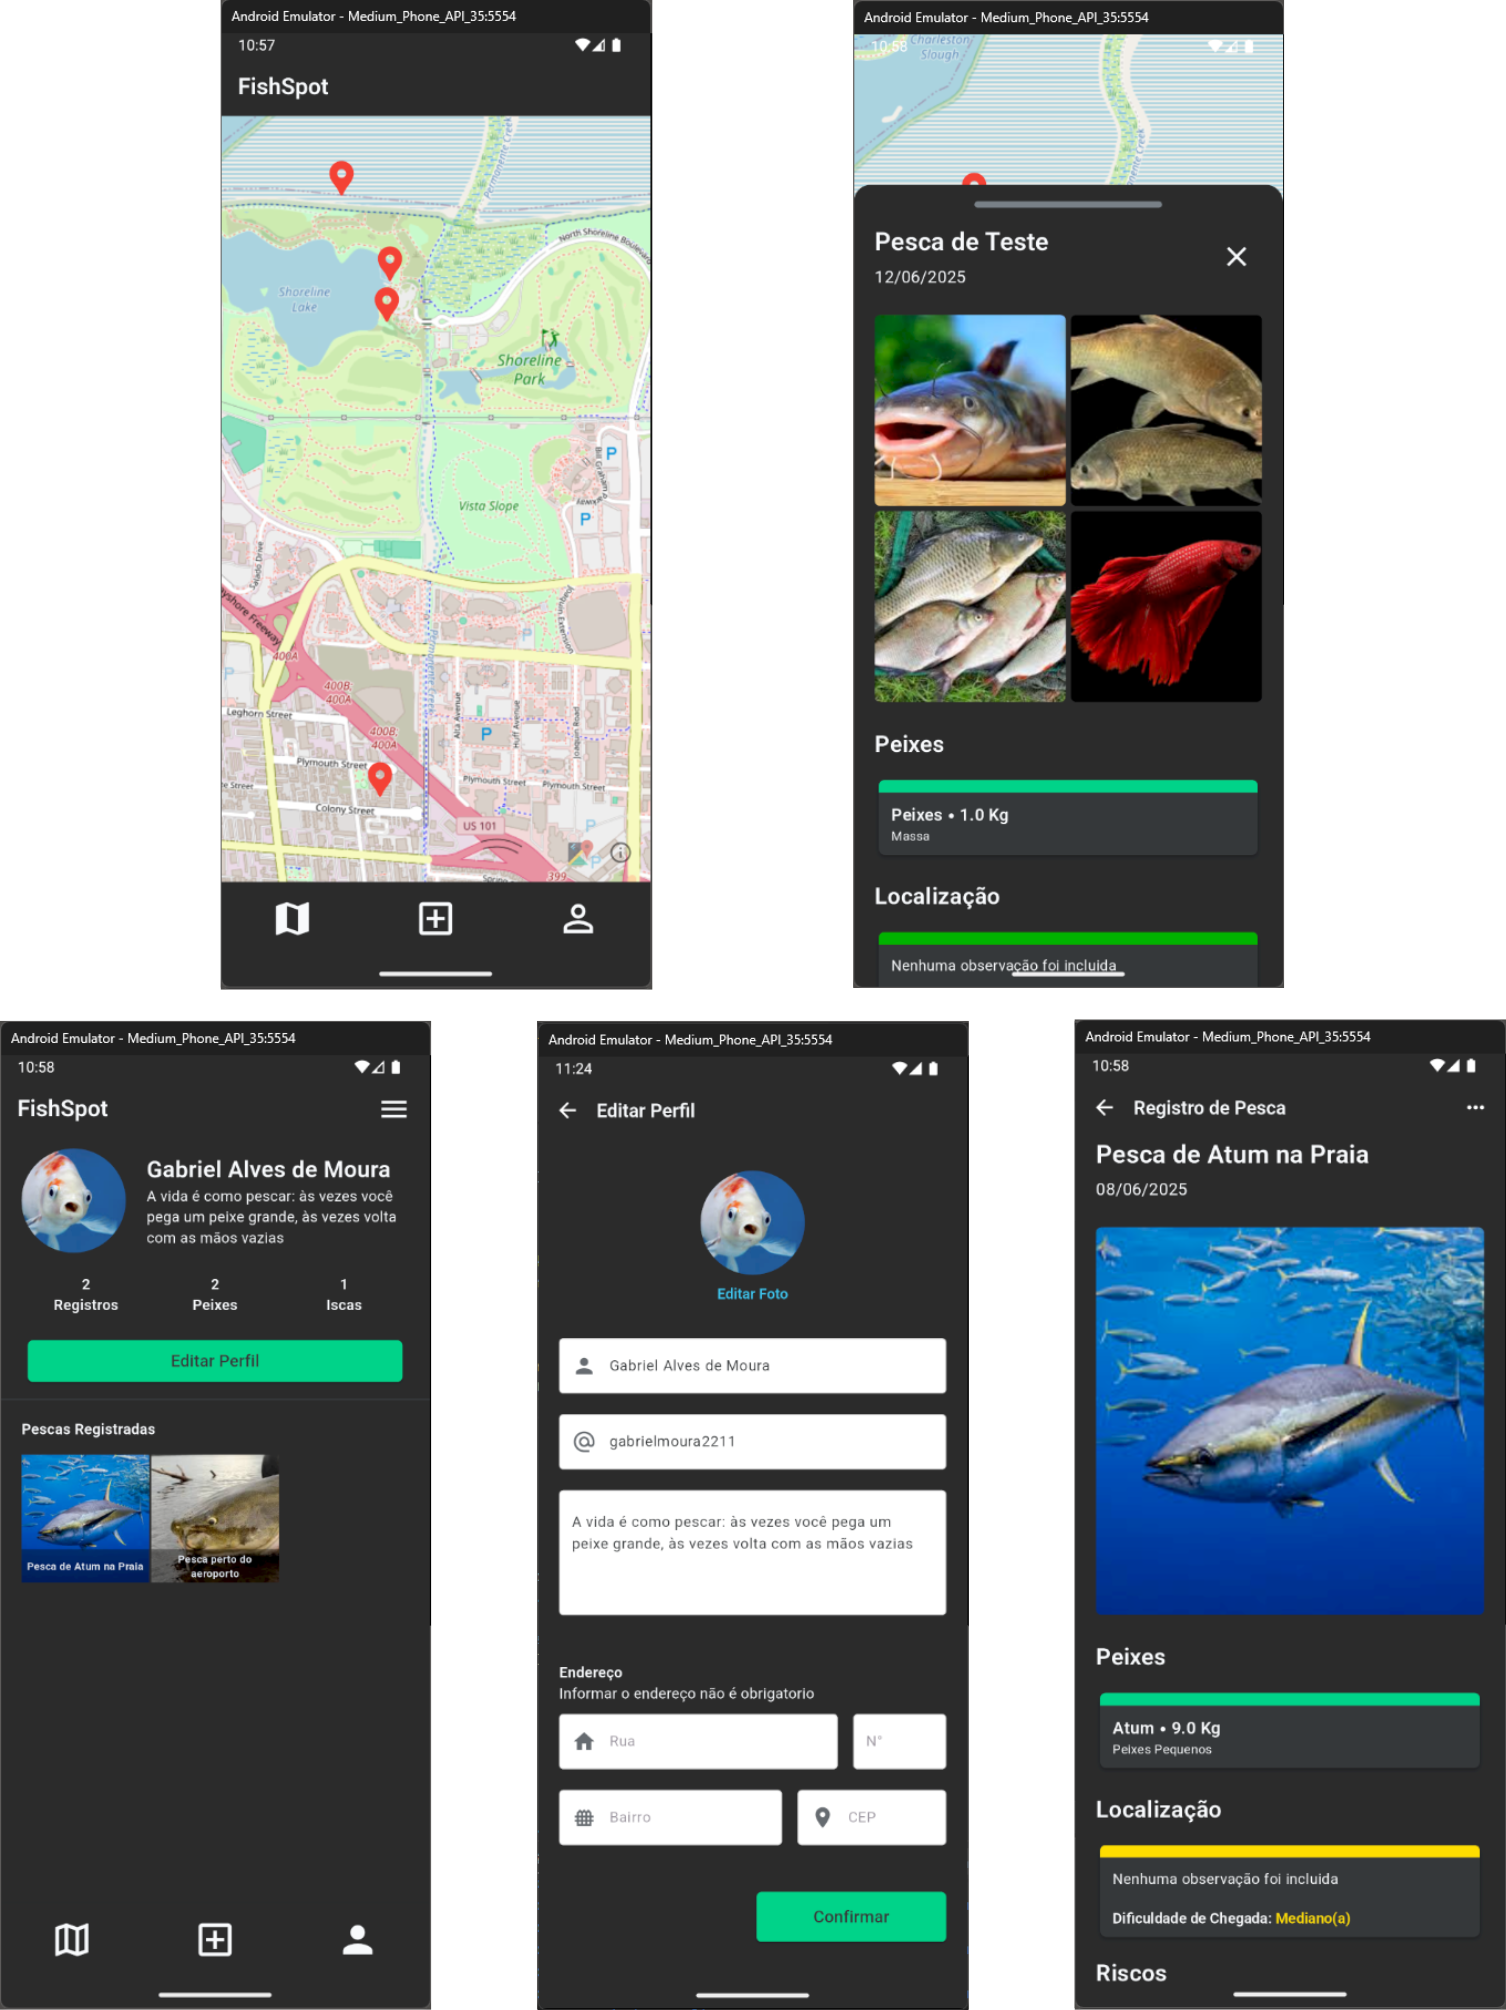
\includegraphics[scale=0.35]{./dados/figuras/emulator-map-and-profile-pages.png}
    \fonte{Produzido pelo Autor}
\end{figure}

O registro de um ponto de pesca está sendo representado pela \autoref{fig:emultatorSpotRegisterPages}, é possivel visualizar as páginas de severidade do local, inclusão de imagens, inclusão de espécies de peixes e descrição do ponto de pesca.

\begin{figure}[H]
    \centering
    \caption{Resultado Obtido - Telas de Registro de Ponto de Pesca}
    \label{fig:emultatorSpotRegisterPages}
    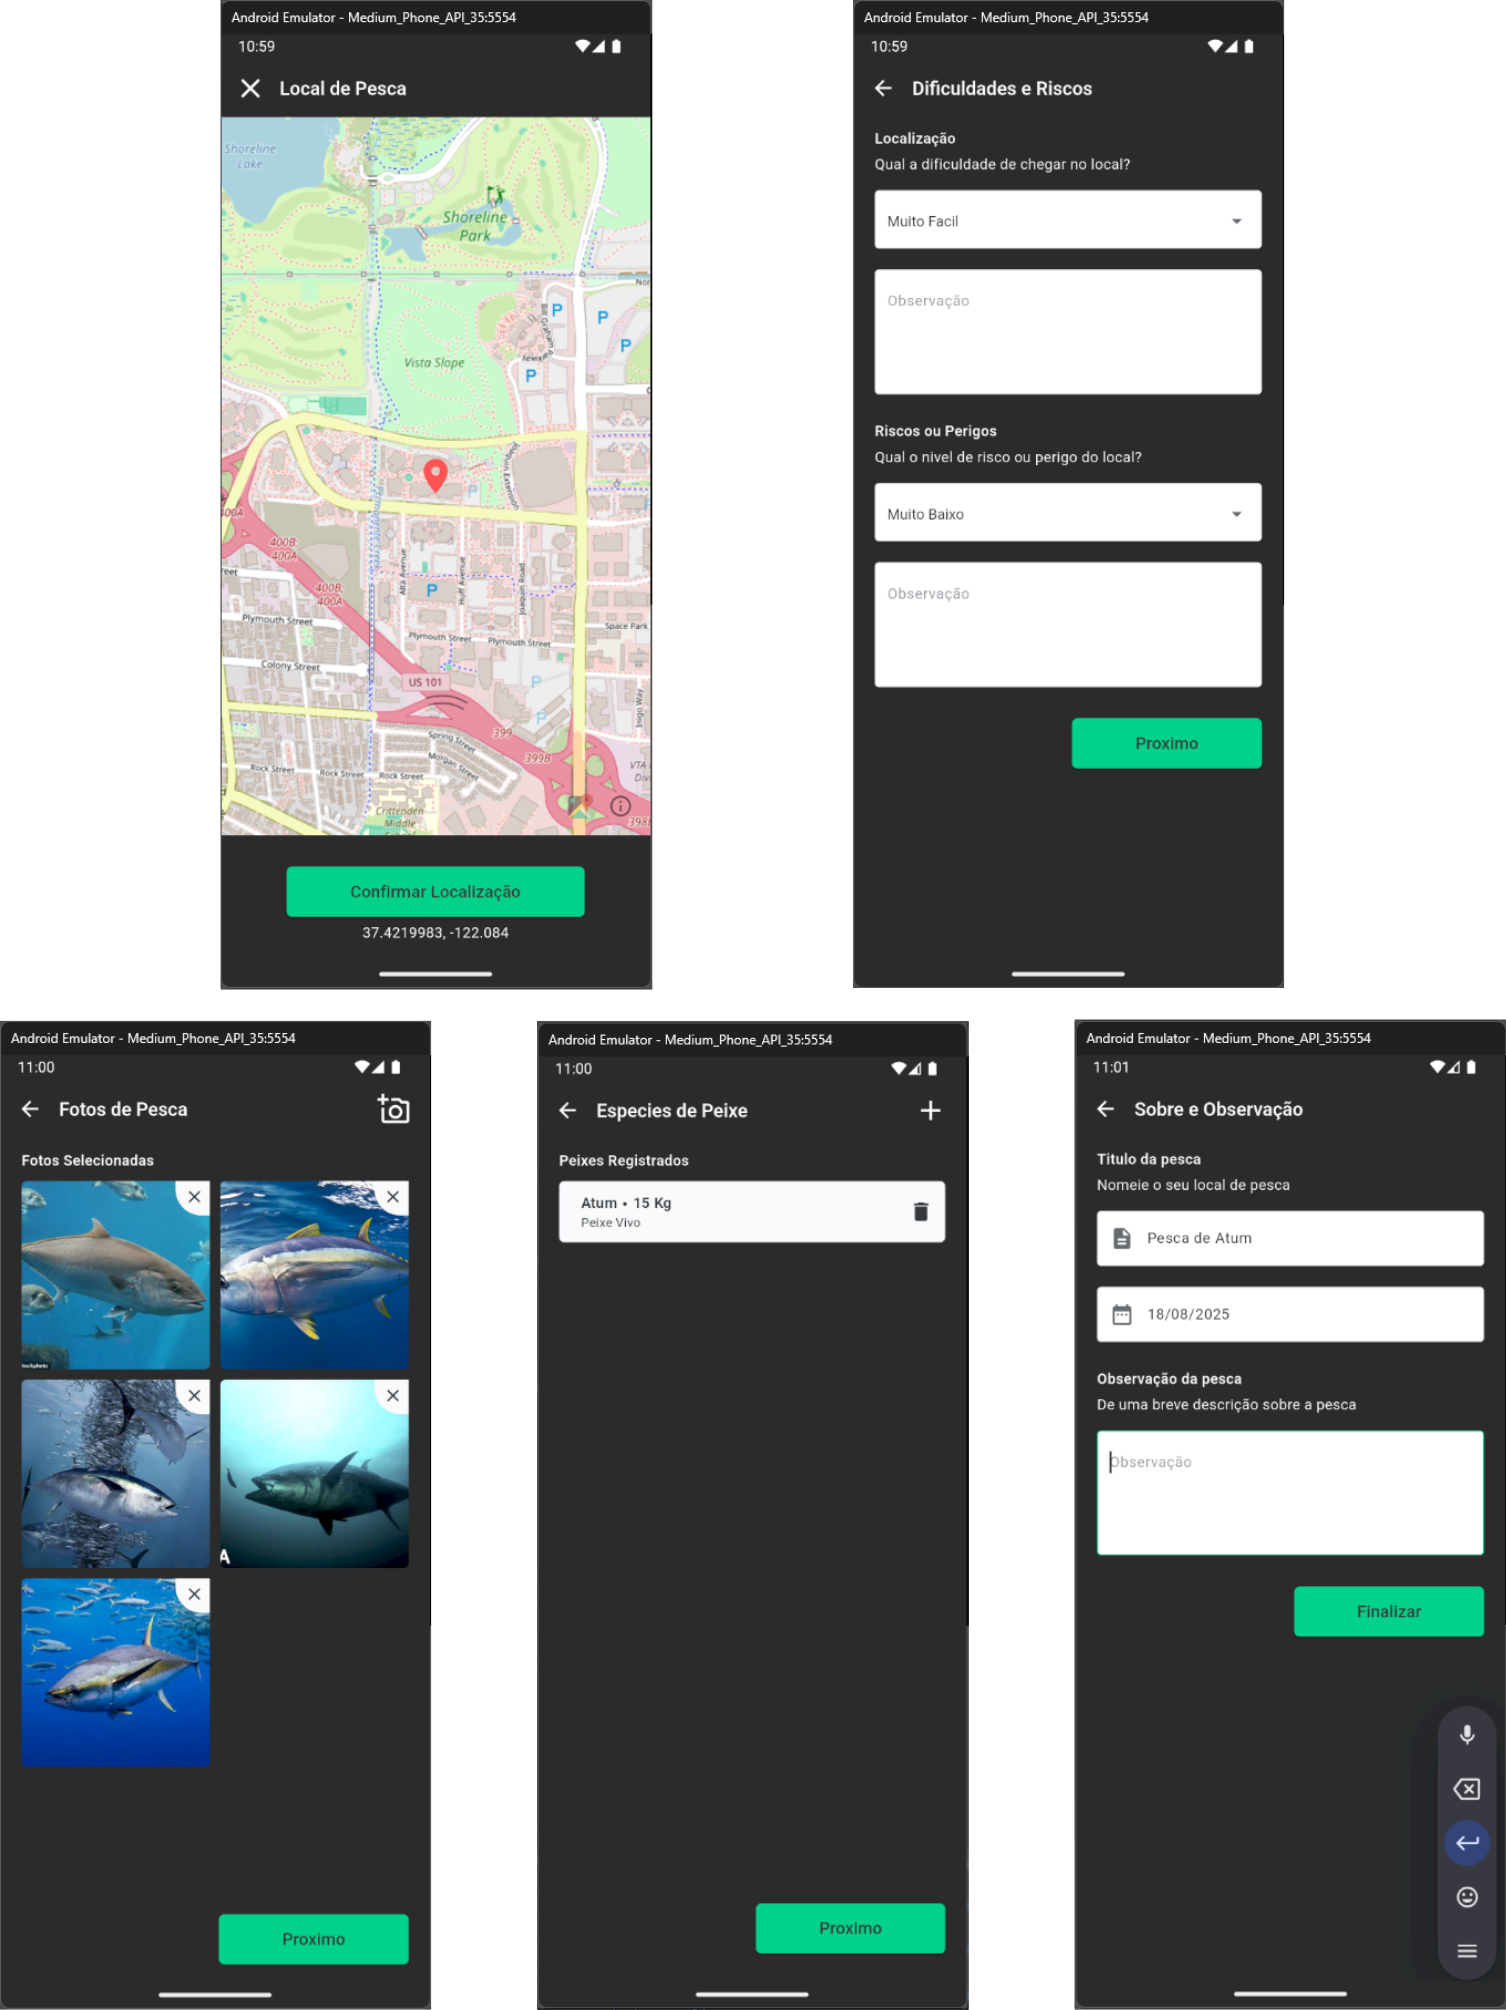
\includegraphics[scale=0.35]{./dados/figuras/emulator-spot-register-pages.png}
    \fonte{Produzido pelo Autor}
\end{figure}

% ---- Modo Claro

A \autoref{fig:emultatorAuthPagesLight} mostra as páginas relacionadas a autenticação do usuário, registro do usuário e recuperação de senha. Todas as telas foram desenvolvidas utilizando o esquema de cores do modo claro.

\begin{figure}[H]
    \centering
    \caption{Resultado Obtido - Telas de Autenticação}
    \label{fig:emultatorAuthPagesLight}
    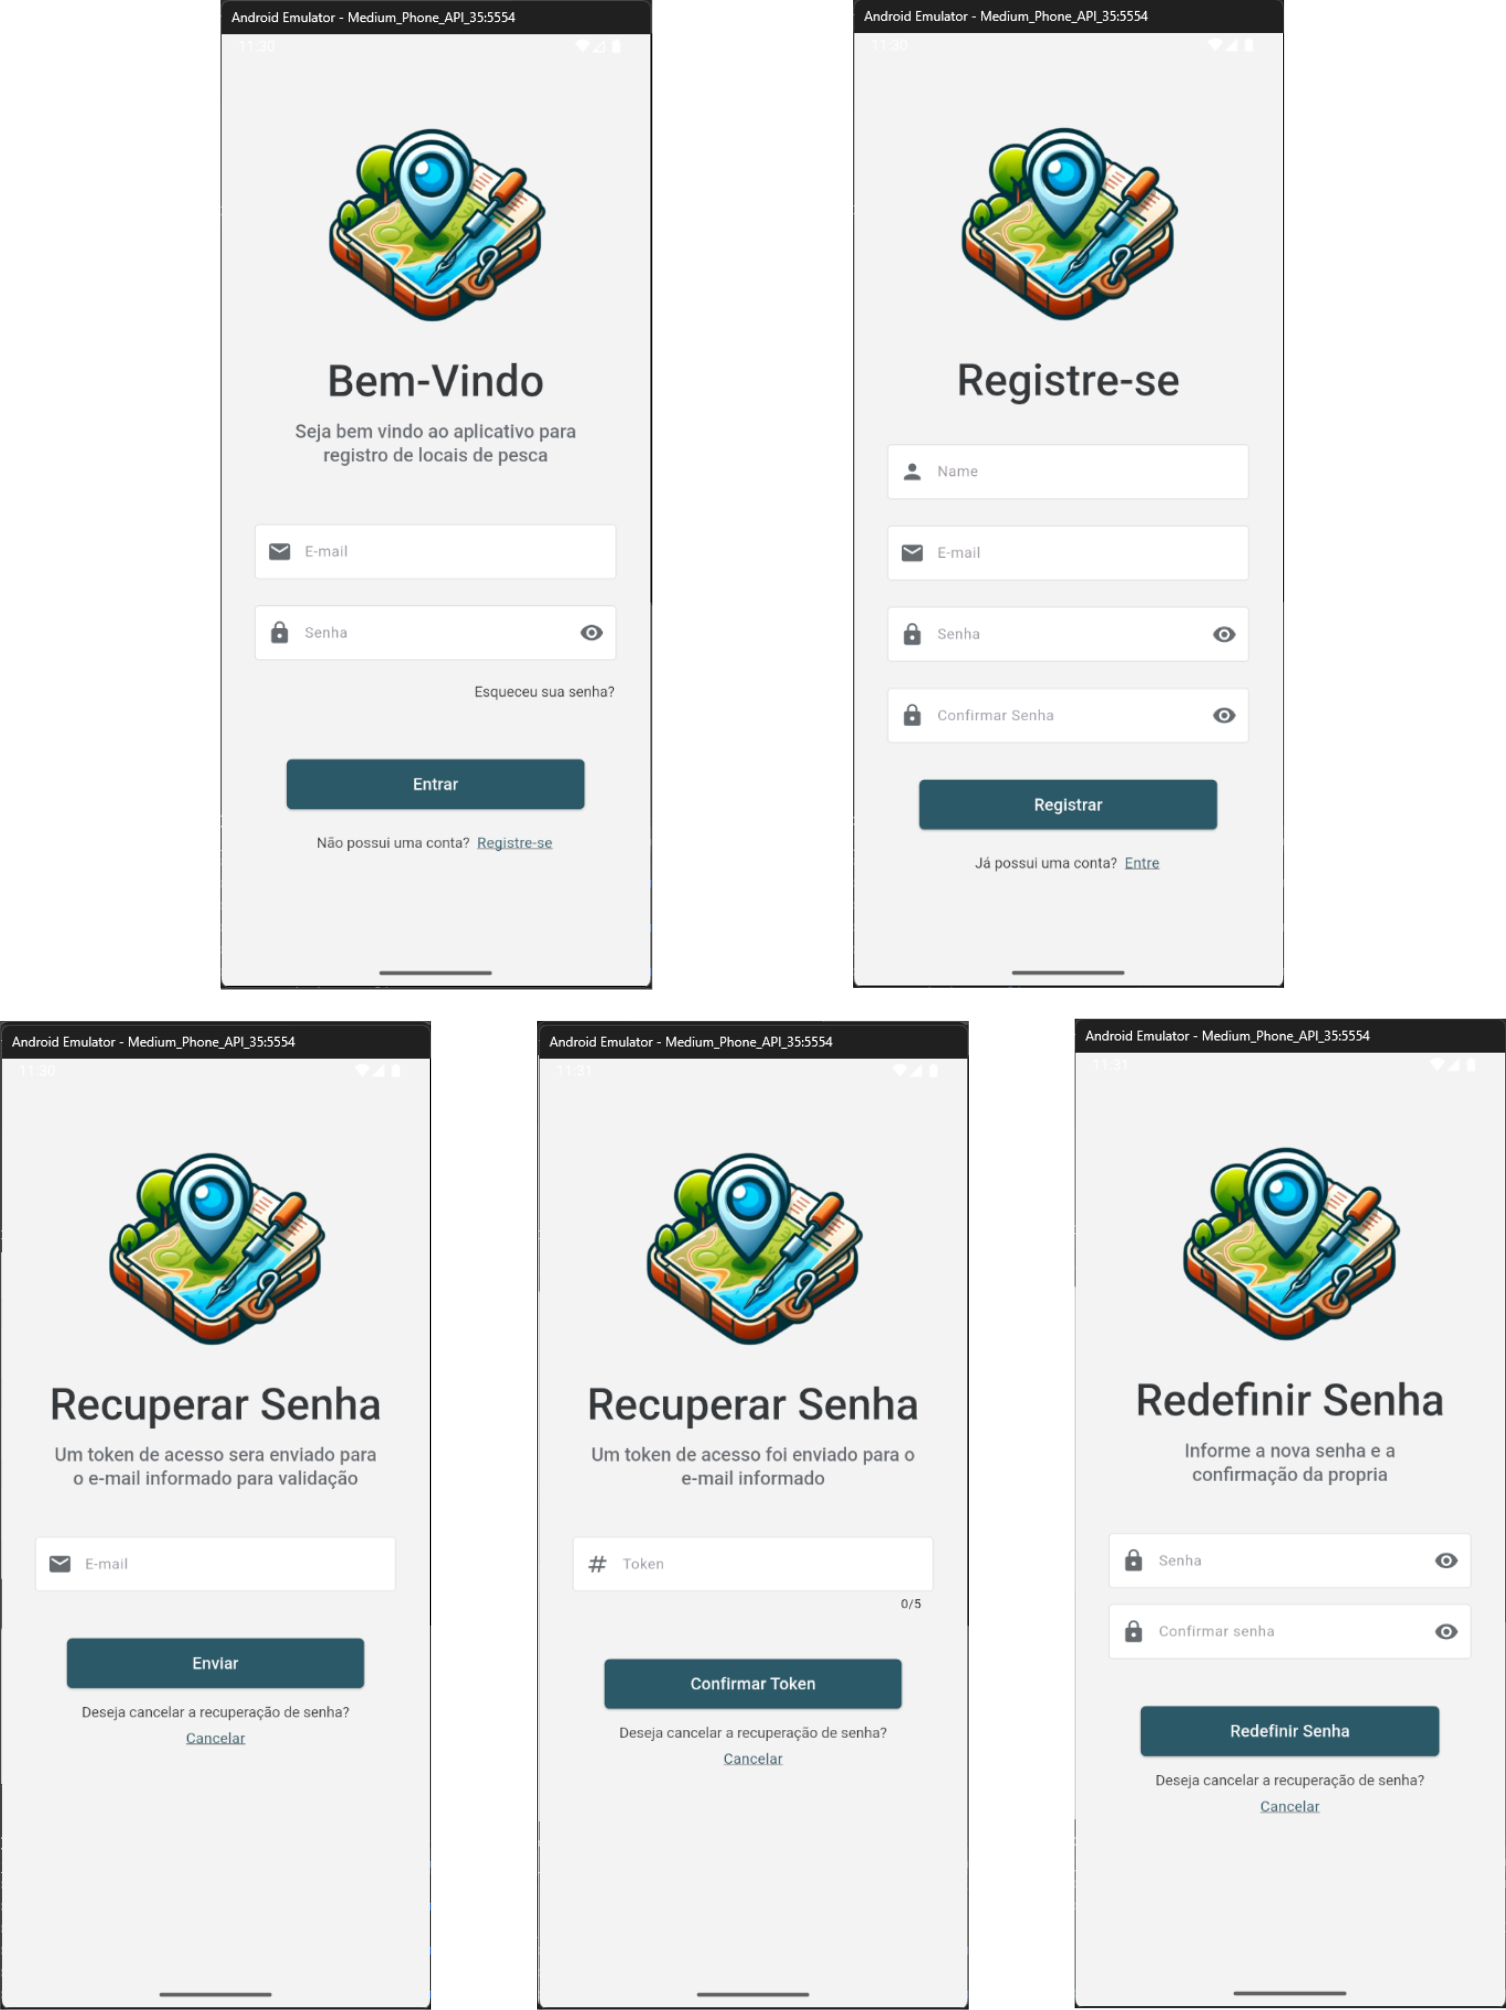
\includegraphics[scale=0.35]{./dados/figuras/emulator-auth-light-pages.png}
    \fonte{Produzido pelo Autor}
\end{figure}


Na \autoref{fig:emultatorMapAndPerfilPagesLight} é possível observar as telas relacionadas ao mapa princpial, detalhes do ponto de pesca, perfil do usuário e tambem edição dos dados do usuário, todas desenvolvidas utilizando esquema de cores do modo claro.

\begin{figure}[H]
    \centering
    \caption{Resultado Obtido - Telas de Mapa e Perfil}
    \label{fig:emultatorMapAndPerfilPagesLight}
    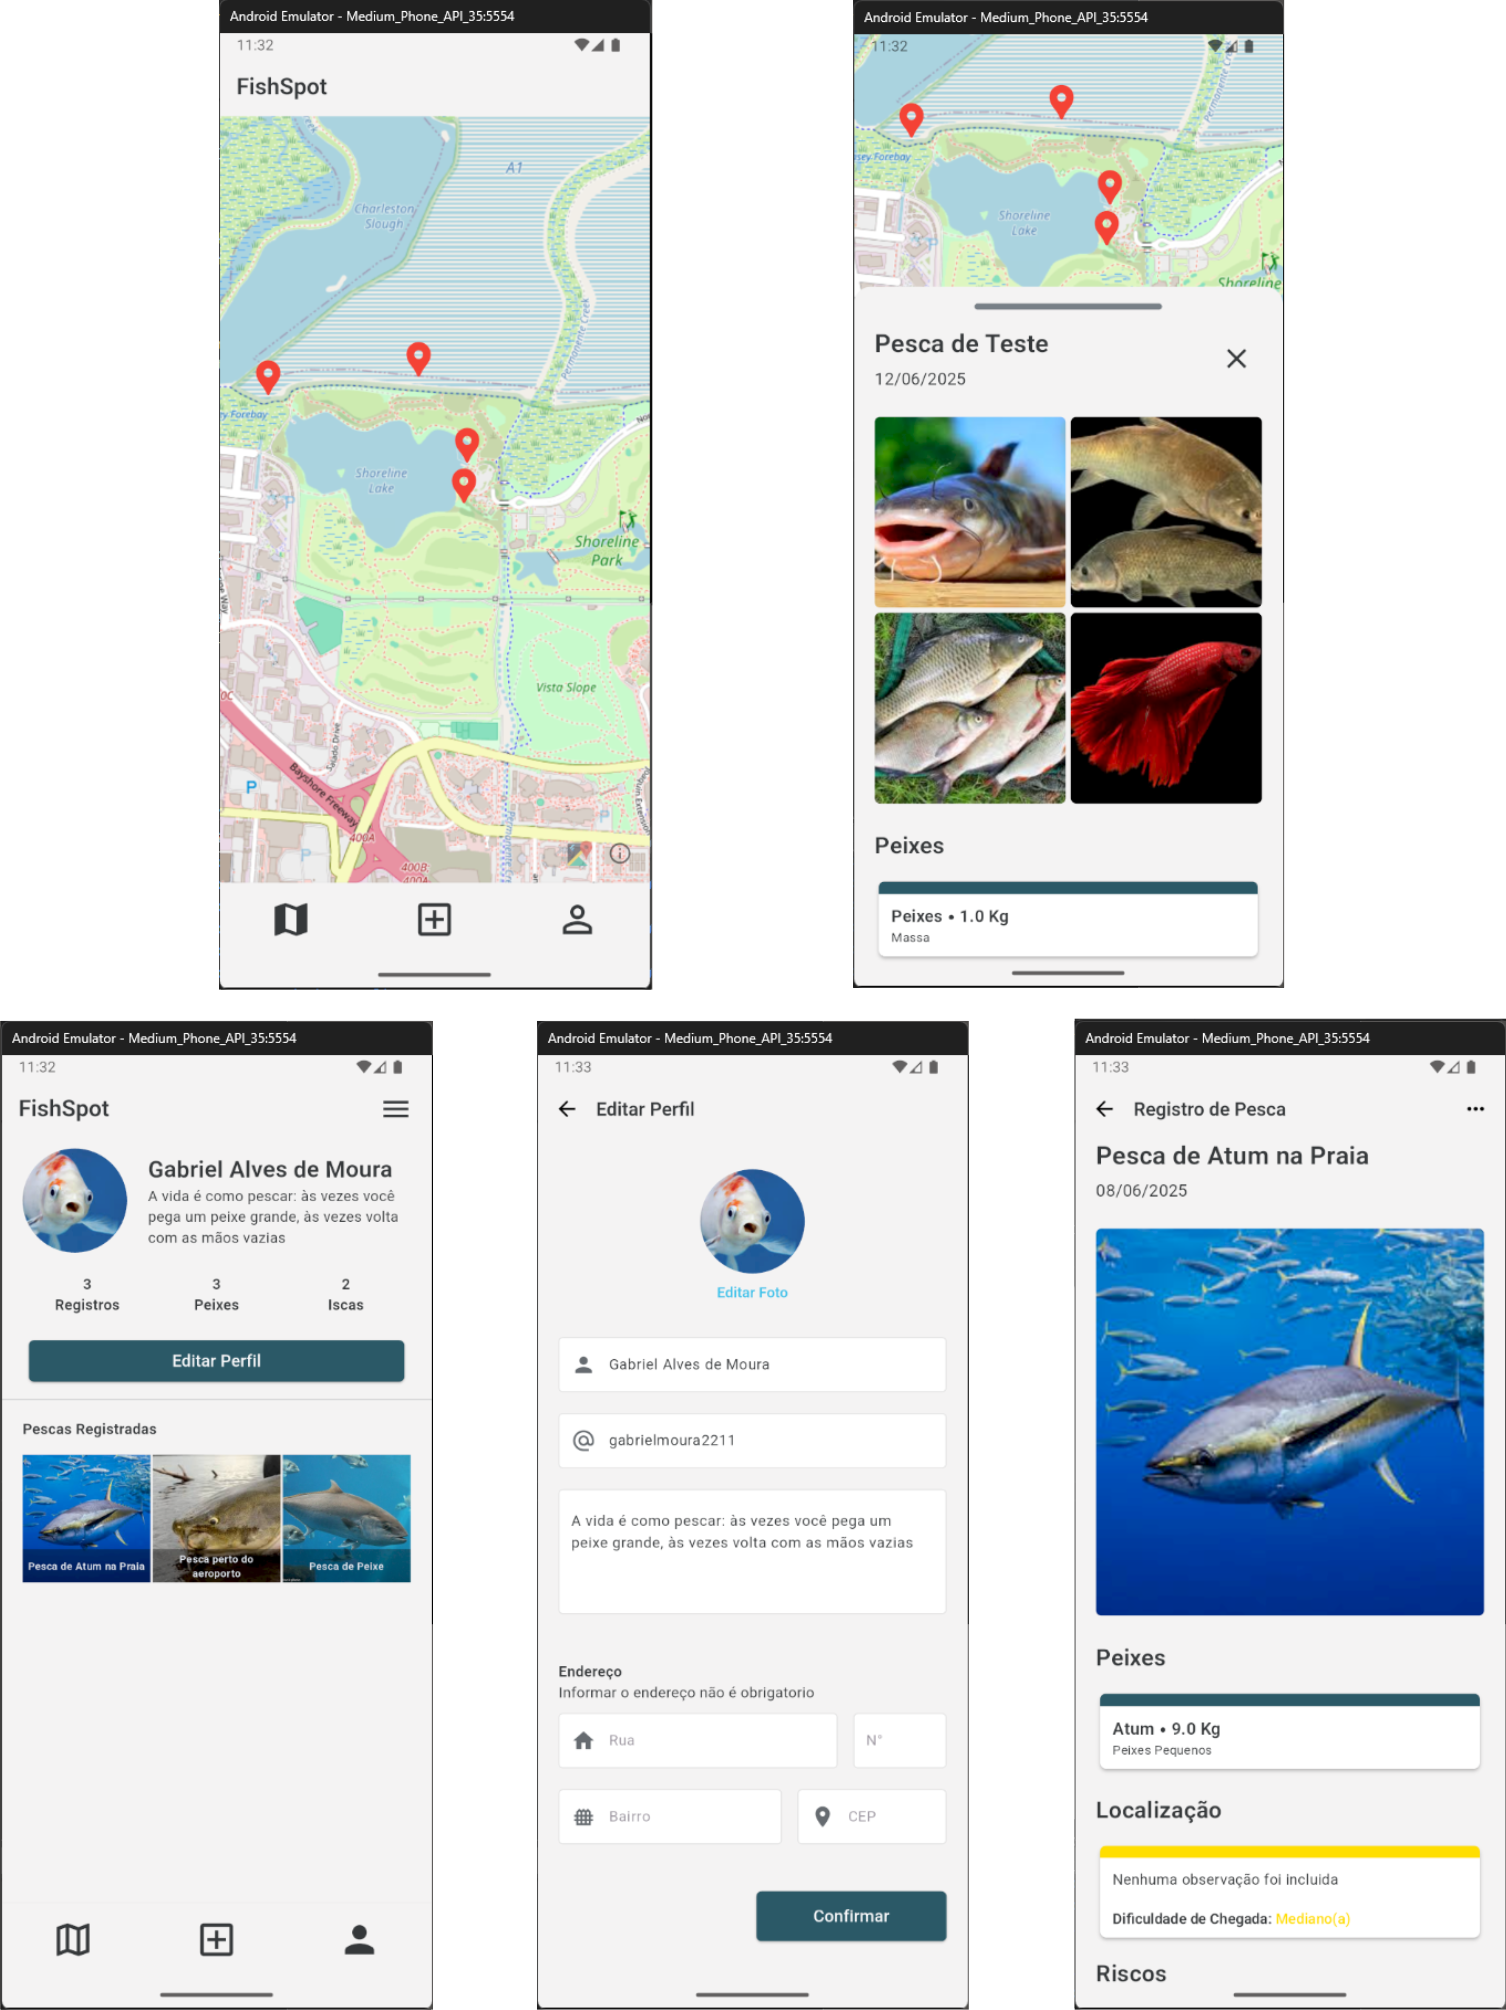
\includegraphics[scale=0.35]{./dados/figuras/emulator-map-and-profile-light-pages.png}
    \fonte{Produzido pelo Autor}
\end{figure}

O registro do ponto de pesca no modo claro está sendo apresentado pela \autoref{fig:emultatorSpotRegisterLightPages}, é possivel observar as telas de confirmação de geolocalização, severidade da localização, inclusão de imagens, inclusão de espécies de peixes e observação do ponto de pesca.

\begin{figure}[H]
    \centering
    \caption{Resultado Obtido - Telas de Registro de Ponto de Pesca}
    \label{fig:emultatorSpotRegisterLightPages}
    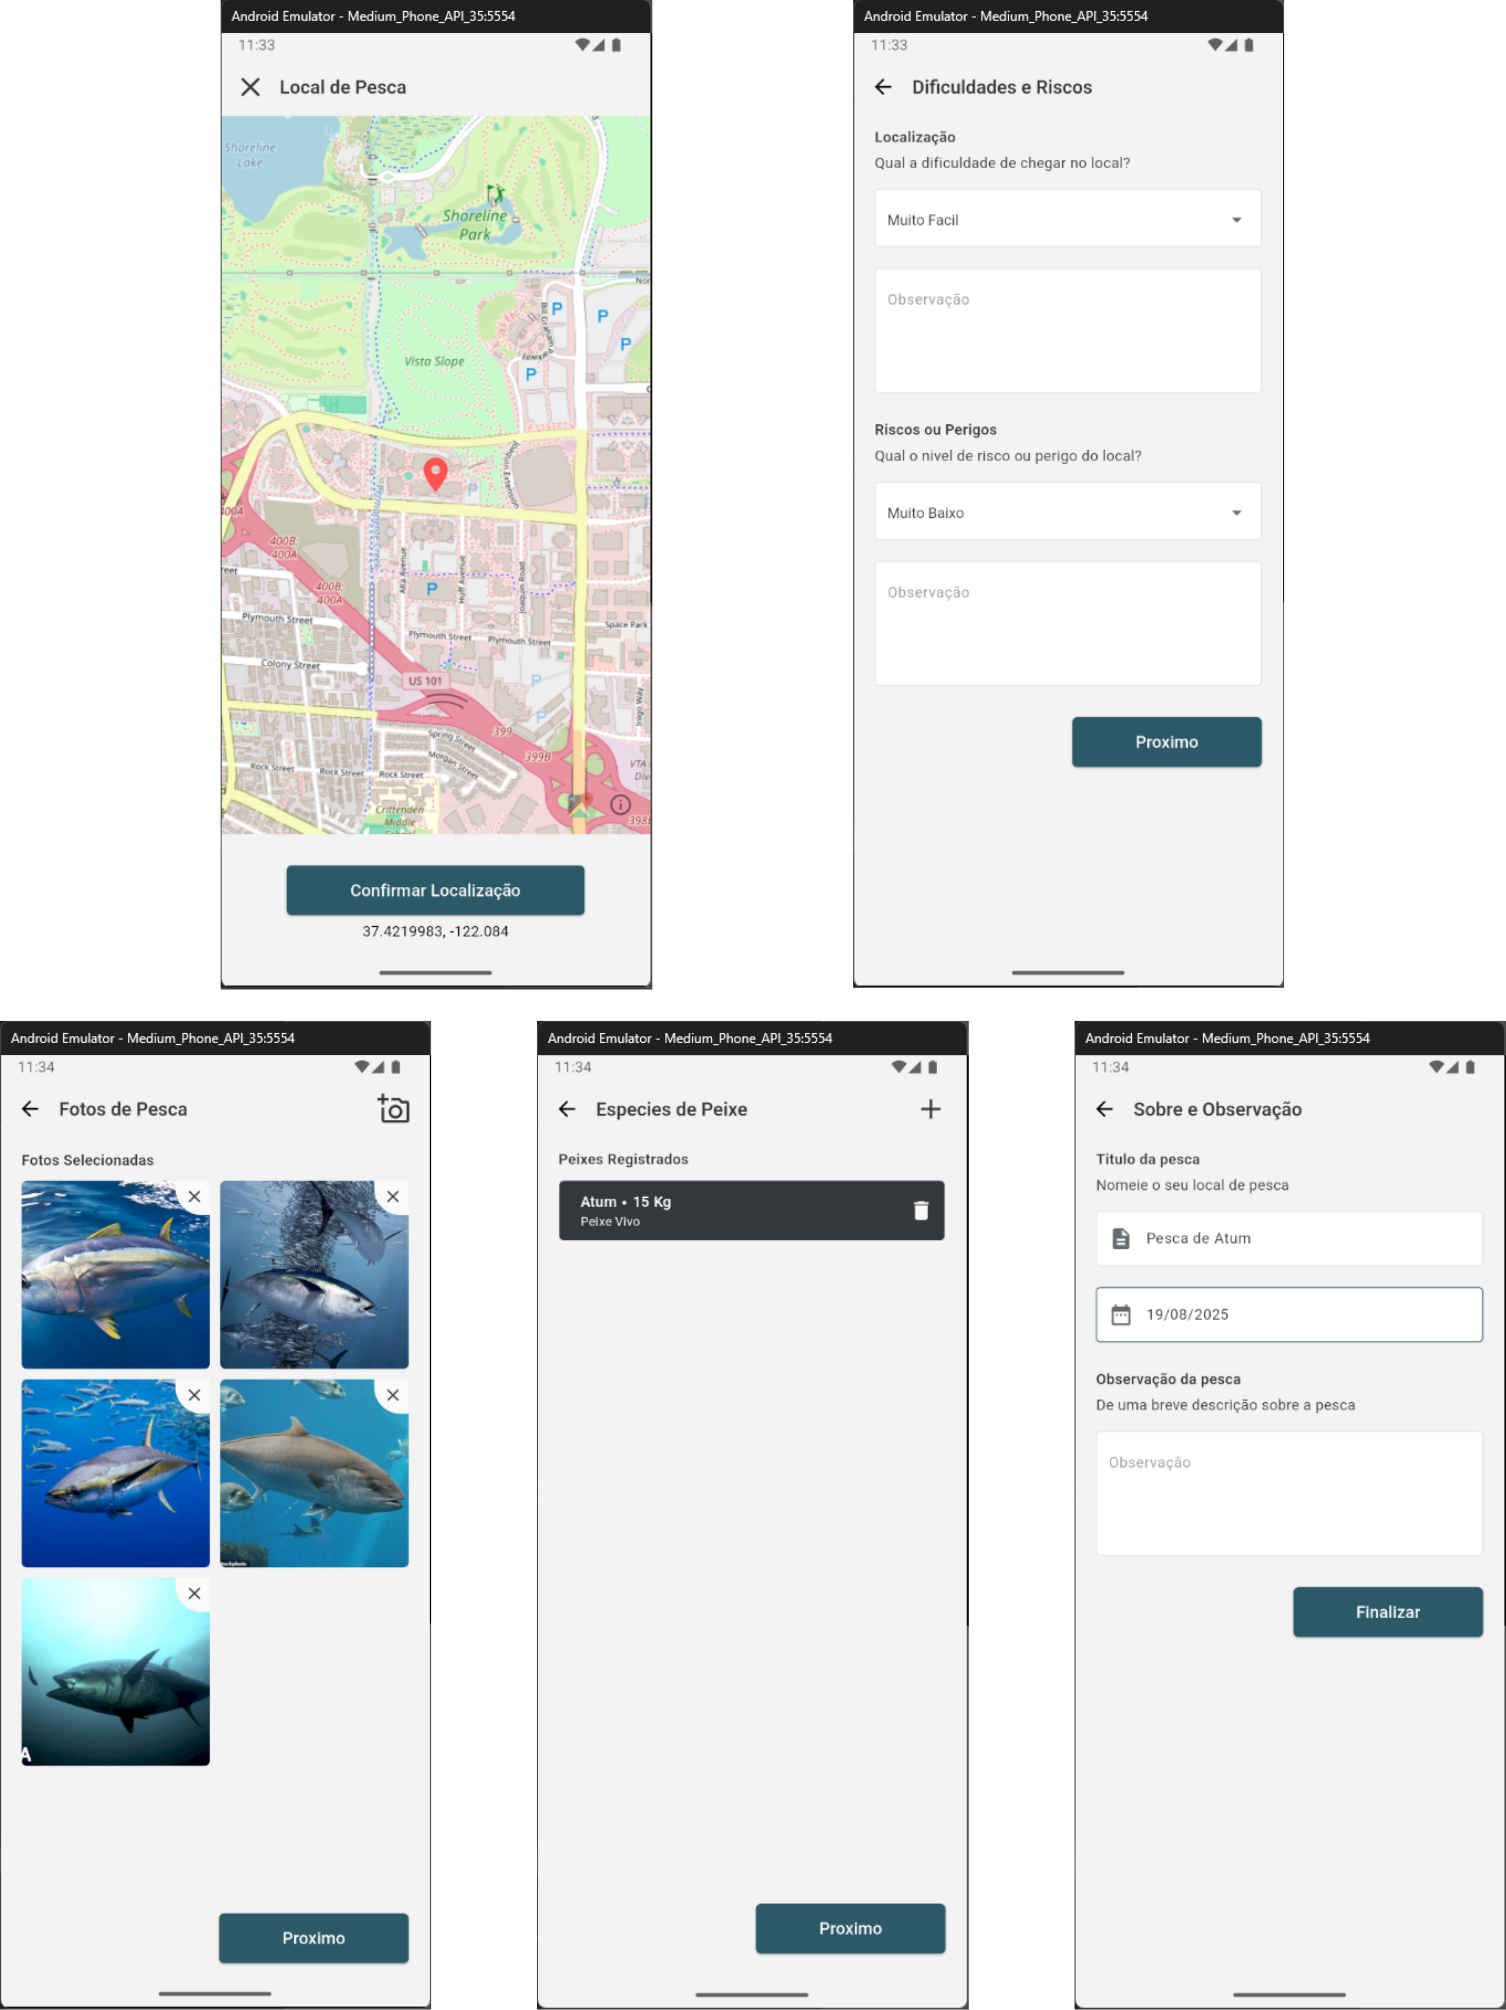
\includegraphics[scale=0.35]{./dados/figuras/emulator-spot-register-light-pages.png}
    \fonte{Produzido pelo Autor}
\end{figure}